\section{Grundlagen}
\sectionbox
{
\subsection{Größen}
\tablebox{
\begin{tabular*}{\columnwidth}{p{4.2cm}cc}
\ctrule
\multicolumn{3}{c}{\textbf{magnetische Größen}}\\
\cmrule
Durchflutung (magnetische Spannungsquelle) & $\Theta$ & $\unitof{\si{\ampere}}$\\
Fluss & $\Phi$ & $\unitof{\si{\voltsecond}}$\\
verketteter Fluss & $\Psi$ & $\unitof{\si{\voltsecond}}$\\
mag. Flussdichte & $\vec{B}$ & $\unitof{\si{\voltsecond\per\metre\squared}}$\\
mag. Feldstärke & $\vec{H}$ & $\unitof{\si{\ampere\per\metre}}$\\
magnetische Spannung & $V_m$ & $\unitof{\si{\ampere}}$\\
magnetischer Widerstand & $R_m$ & $\unitof{\si{\ampere\per\voltsecond}}$\\
Streuziffer & $\sigma$ & $\unitof{\si{1}}$\\
\cmrule
\multicolumn{3}{c}{\textbf{elektrische Größen}}\\
\cmrule
Stromdichte & $\vec{s}$ & $\unitof{\si{\ampere\per\metre\squared}}$\\
dielektrische Verschiebung & $\vec{D}$ & $\unitof{\si{\amperesecond\per\metre\squared}}$\\
el. Feldstärke & $\vec{E}$ & $\unitof{\si{\volt\per\metre}}$\\
Strombelag & $a$ & $\unitof{\si{\ampere\per\metre}}$\\
spezifischer Widerstand & $\rho$ & $\unitof{\si{\ohm\meter}}$\\
\cmrule
\multicolumn{3}{c}{\textbf{mechanische Größen}}\\
\cmrule
Drehmoment & $M$ & $\unitof{\si{\newtonmeter}}$\\
Massenträgheitsmoment & $J$ & $\unitof{\si{\kilo\gram\metre\squared}}$\\
Spulenwindungszahl & $w_\text{Sp}$ & $\unitof{1}$\\
effektive Windungszahl & $w_\text{eff}$ & $\unitof{\si{1}}$\\
Luftspalthöhe & $\delta$ & $\unitof{\si{\milli\meter}}$\\
scheinbarer Luftspalt & $\delta'$ & $\unitof{\si{\milli\meter}}$\\
effektiver Luftspalt & $\delta''$ & $\unitof{\si{\milli\meter}}$\\
Anzahl der Leiter pro Nut & $Z_N$ & $\unitof{\si{1}}$\\
Zahl der Einzelspulen (Kommutatorsegmente) & $Z_K$ & $\unitof{\si{1}}$\\
ideelle Eisenlänge & $l_i$ & $\unitof{\si{\meter}}$\\
bewickelbare Nutfläche & $A_N$ & $\unitof{\si{\meter\squared}}$\\
magnetisch aktiver Winkel & $\beta_M$ & $\unitof{\si{\radian}}$\\
Drehzahl & $n$ & $\unitof{\si{\per\second}}$\\
Rotornutenzahl & $N$ & $\unitof{\si{1}}$\\
Rotornutenzahl pro Pol & $Q$ & $\unitof{\si{1}}$\\
Anzahl paralleler Zweige & $a$ & $\unitof{\si{1}}$\\
\cmrule
\multicolumn{3}{c}{\textbf{Näherungsfaktoren}}\\
\cmrule
Carterfaktor & $k_C$ & $\unitof{\si{1}}$\\
Eisenfüllfaktor & $k_\text{Fe}$ & $\unitof{\si{1}}$\\
Eisenfaktor (Magnnetisierungsbedarf Eisen) & $k_\mu$ & $\unitof{\si{1}}$\\
Nutfüllfaktor & $k_Q$ & $\unitof{\si{1}}$\\
\cbrule
\end{tabular*}
}
}
\sectionbox{
\symbolbox{
\begin{tabularx}{\columnwidth}{lX}
Permeabilität & $\mu_0 = \SI{4\pi e-7}{\volt\second\per\ampere\metre}$ \\
Permittivität & $\varepsilon_0 = \SI{8,854e-12}{\ampere\second\per\volt\metre}$
\end{tabularx}
}
\subsubsection{Allgemeine Maschinenbegriffe - Durchmesser}
\mbox{
\pbox[c]{4cm}{
    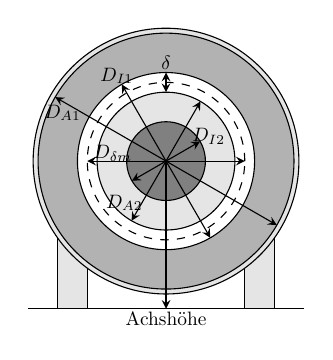
\begin{tikzpicture}[scale=.5,every node/.style={scale=.7} , >=stealth]
	\draw (-3.5,-3.75) -- (3.5,-3.75);

	\filldraw[fill=black!10!white, draw=black]
		(-2.75,-3.75) rectangle (-2.0,0);
	\filldraw[fill=black!10!white, draw=black]
		(2.75,-3.75) rectangle (2.0,0);
	
	\filldraw[fill=black!10!white, draw=black]
		(0,0) circle (3.375 cm);
	\filldraw[fill=black!30!white, draw=black]
		(0,0) circle (3.25 cm);
	\filldraw[fill=white, draw=black]
		(0,0) circle (2.25 cm);
	\draw [dashed] (0,0) circle (2.0 cm);
	\filldraw[fill=black!10!white, draw=black]
		(0,0) circle (1.75 cm);
	\filldraw[fill=black!50!white, draw=black]
		(0,0) circle (1 cm);
		
	% Achshöhe
	\draw [->] (0,0) -- (0,-3.75);
	\draw (0, -4) node {Achshöhe}; 
	
	% D_\delta m
	\draw [<->] (-2,0) -- (2,0); 
	\draw (-1.35,0.2) node {$D_{\delta\text m}$};

	% delta
	\draw [<->] (0,1.75) -- (0,2.25);
	\draw (0,2.5) node {$\delta$};

	% D_I2
	\draw [<->] (210:1) -- (30:1);
	\draw (30:1.25) node {$D_\text{I2}$};

	% D_A1
	\draw [<->] (150:3.25) -- (330:3.25);
	\draw (155:2.9) node {$D_\text{A1}$};
	
	% D_A2
	\draw [<->] (60:1.75) -- (240:1.75);
	\draw (225:1.5) node {$D_\text{A2}$}; 

	% D_I1
	\draw [<->] (120:2.25) -- (300:2.25);
	\draw (120:2.5) node {$D_\text{I1}$}; 
	
\end{tikzpicture}
	}
	}
\begin{minipage}{3cm}
	\tablebox{
	\begin{tabularx}{\columnwidth}{l c}
		\ctrule
		\multicolumn{2}{c}{\textbf{Maße}}\\
		\cmrule
		Stator Außend. & $D_\text{A1}$\\
		Stator Innend. & $D_\text{I1}$\\
		Rotor Außend. & $D_\text{A2}$\\
		Rotor Innend. & $D_\text{I2}$\\
		\cmrule
		\multirow{2}{*}{Mittl. Luftspaltd.} & $D$\\
		& $D_{\delta\text m}$\\
		\cmrule
		Luftspalthöhe & $\delta$\\
		\cbrule
	\end{tabularx}
	}
\end{minipage}

\subsubsection{Allgemeine Maschinenbegriffe - Abmessungen}
\mbox{
\pbox[c]{4cm}{
    \begin{tikzpicture}[scale=.5,every node/.style={scale=.7} , >=stealth]
	
	\filldraw[fill=black!10!white, draw=black] 
		(0,0) circle (3.5 cm);
	
	\filldraw[fill=white, draw=black] 
		(105:3.0) arc (105:255:3.0) 
		-- ++(0,1) -- (225:1.75) arc (225:315:1.75) 
		-- ($(285:3.0) + (0,1)$) -- ++(0,-1) arc (-75:75:3.0) 
		-- +(0,-1) -- (45:1.75) arc (45:135:1.75)
		-- ($(105:3.0) + (0,-1)$) -- cycle;

	\draw[draw=black!10!white]
		(-2.98,0) -- (2.98,0);
	
	\draw[draw=black!10!white]
		(0,0) -- (225:1.73);
	
	\coordinate (a1) at (5:1.5);
	\coordinate (i1) at ($(5:1.5) + (-0.707,0)$);
	\coordinate (i2) at ($(40:1.5) + (-0.5,-0.5)$);
	\coordinate (i3) at ($(50:1.5) + (-0.5,-0.5)$);
	\coordinate (i4) at ($(85:1.5) - (0,0.707)$);
	\coordinate (i5) at ($(95:1.5) - (0,0.707)$);
	\coordinate (i6) at ($(130:1.5) - (-0.5,0.5)$);
	\coordinate (i7) at ($(140:1.5) - (-0.5,0.5)$);
	\coordinate (i8) at ($(175:1.5) - (-0.707,0)$);
	\coordinate (i9) at ($(185:1.5) - (-0.707,0)$);
	\coordinate (i10) at ($(220:1.5) - (-0.5,-0.5)$);
	\coordinate (i11) at ($(230:1.5) - (-0.5,-0.5)$);
	\coordinate (i12) at ($(265:1.5) - (0,-0.707)$);
	\coordinate (i13) at ($(275:1.5) - (0,-0.707)$);
	\coordinate (i14) at ($(310:1.5) - (0.5,-0.5)$);
	\coordinate (i15) at ($(320:1.5) - (0.5,-0.5)$);
	\coordinate (i16) at ($(355:1.5) - (0.707,0)$);
	\coordinate (b1) at ($(85:1.5) - (0,0.8)$);
	\coordinate (b2) at ($(95:1.5) - (0,0.8)$);
	
	\filldraw[fill=black!10!white, draw=black] 
		(i1) -- (a1) 
		arc (5:40:1.5) -- (i2) -- (i3) -- ++(0.5,0.5) 
		arc (50:85:1.5) -- (i4) -- (i5) -- ++(0,0.707)
		arc (95:130:1.5) -- (i6) -- (i7) -- ++(-0.5,0.5)
		arc (140:175:1.5) -- (i8) -- (i9) -- ++(-0.707,0)
		arc (185:220:1.5) -- (i10) -- (i11) -- ++(-0.5,-0.5)
		arc (230:265:1.5) -- (i12) -- (i13) -- ++(0,-0.707)
		arc (275:310:1.5) -- (i14) -- (i15) -- ++(0.5,-0.5)
		arc (320:355:1.5) -- (i16) -- cycle;

	\filldraw[fill=white, draw=black]
		(0,0) circle (0.35cm);

	% h_j
	\draw [<->] (130:3.5) -- (130:3);
	\draw (125:3.25) node {$h_\text{J}$};  
	
	% Beschriftung
	\draw (60:3.25) node {Joch};
	\draw (0, 2.25) node {Pol};
	\draw (0, -2.25) node {Pol};
	
	\draw [<-] (23:1.2) -- (21:2.0);
	\draw (23:2.3) node {Zahn};
	
	\draw [<-] (315:1.5) -- ++(0.7,-0.1);
	\draw (315:1.5) ++(0.7,-0.1) ++(0.3,0) node {Nut};
	
	% Hilfslinien
	\draw[draw=black!10!white]
		(-0.33,0) -- (0.33,0);
	\draw[draw=black!10!white]
		(0,0) -- (225:0.33);
	
	% tau_N
	\draw [<->, very thin] (180:1.625) arc (180:225:1.625);
	\draw (202:1.85) node {$\tau_\text N$};

	% tau_p
	\draw [<->, very thin] (0:1.625) arc (0:180:1.625);
	\draw (155:1.85) node {$\tau_p$};
	
	% b_N
	\draw [very thin] (i4) -- (b1);
	\draw [very thin] (i5) -- (b2);
	\draw (0,0.5) node {$b_\text{N}$};	
	
	% h_N
	\draw [very thin] (95:1.5) -- +(-0.2,0);
	\draw [very thin] (i5) -- +(-0.2,0);
	\draw (108:1.2) node {$h_\text{N}$};
	
	
\end{tikzpicture}
	}
	}
\begin{minipage}{3cm}
	\tablebox{
	\begin{tabularx}{\columnwidth}{l c c}
		\ctrule
		\multicolumn{3}{c}{\textbf{Maße}}\\
		\cmrule
		Nutzahl & $N$ & $\unitof{\si{1}}$\\
		Nutteilung & $\tau_N$ & $\unitof{\si{\centi\metre}}$\\
		\cmrule
		Polpaarzahl & $p$ & $\unitof{\si{1}}$ \\
		Polteilung & $\tau_p$ & $\unitof{\si{\centi\metre}}$\\
		\cmrule
		Nuthöhe & $h_N$ & $\unitof{\si{\centi\metre}}$\\
		Nutbreite & $b_N$ & $\unitof{\si{\centi\metre}}$\\
		Jochhöhe & $h_J$ & $\unitof{\si{\centi\metre}}$\\
		\cbrule
	\end{tabularx}
	\begin{tabularx}{\columnwidth}{c c}
		\ctrule
		$\tau_N = \frac{\pi\cdot D}{N}$ & $\tau_p = \frac{\pi\cdot D}{2p}$\\
		\cbrule
	\end{tabularx}
	}
\end{minipage}
}
\sectionbox{
\subsection{Grundlegende Gleichungen}
\subsubsection{Maxwell}

\begin{tabularx}{\columnwidth}{>{\centering\arraybackslash}m{0.435\columnwidth}|>{\centering\arraybackslash}m{0.435\columnwidth}}
$\rot \vec{H} = \vec{s} + \frac{\partial\vec{D}}{\partial t}$  & \multirow{2}{*}{$\rot\vec{E} = - \frac{\partial\vec{B}}{\partial t}$} \\
$\rot \vec{H} = \vec{s} \quad (< 10\si{\kilo\hertz})$ & \\
\hline
\multirow{2}{*}{$\div\vec B = 0$} & \multirow{2}{*}{$\div\vec D = \gamma$} \\
 & \\
\end{tabularx}

\subsubsection{Durchflutungs- und Induktionsgesetz}
\begin{tabularx}{\columnwidth}{>{\centering\arraybackslash}m{0.435\columnwidth}|>{\centering\arraybackslash}m{0.435\columnwidth}}
\textbf{Durchflutungsgesetz} & \textbf{Induktionsgesetz}\\
\hline
\vspace{3pt}$\oint_{L_A}\vec{H}\diff\vec{l} = \iint_{A_L}\vec{s}\diff\vec{A} = \Sigma i = \Theta$ & \vspace{3pt}\mbox{$u_i = \frac{\partial\Psi(t)}{\partial t} = \frac{\partial}{\partial t}\left(\iint_A \vec{B}\diff\vec{A}\right)$}
$\oint_L \vec{E}\diff\vec{l} + u_\text{i} = 0$\\
\end{tabularx}

\subsubsection{Kenngrößen}
\begin{tabularx}{\columnwidth}{>{\centering\arraybackslash}m{0.435\columnwidth}|>{\centering\arraybackslash}m{0.435\columnwidth}}
\textbf{magnetische Größen} & \textbf{elektrische Größen}\\
\hline
\vspace{3pt}$\Phi = \iint\vec{B}\diff\vec{A}$ & \vspace{3pt}$I = \iint\vec{s}\diff\vec{A}$\\
$V_m = \int \vec{H}\diff\vec{l}$ & $U = \int \vec{E}\diff\vec{l}$\\
$\Theta = w\cdot I$ & \\
$R_m = \frac{V_m}{\Phi} = \frac{l}{\mu\cdot A}$ & $R = \frac{U}{I} = \rho\frac{l}{A}$\\
$\vec{B} = \mu\cdot\vec{H}$ & $\vec{D} = \varepsilon\cdot \vec{E}$\\
$\Psi = \Phi\cdot w = L\cdot i$ & \\
\vspace{3pt}
\begin{circuitikz}[scale=.8, transform shape, font=\large]
\draw	(0,2) to [short, i=$\Phi$] (1.5,2)
			to [R, l_=$R_\text{m}$,v^>=$V$](1.5,0)
			to (0,0)
			to [V<=$\Theta$](0,2);
\end{circuitikz} & \vspace{3pt}
\begin{circuitikz}[scale=.8, transform shape, font=\large]
\draw	(4,2) to [short, i=$I$] (5.5,2)
			to [R, l_=$R$,v^>=$U$](5.5,0)
			to (4,0)
			to [V<=$U$](4,2);
\end{circuitikz}\\
magnetisch wirksame Fläche & \\
$A = k_\text{Fe}\cdot A_\text{geometrisch}$
\end{tabularx}
}
\sectionbox{
\subsection{Entstehung des Drehmoments}
\subsubsection{Lorenzkraft}

\[\vec{F_L} = I\cdot (\vec{l}\times \vec{B})\]

\subsubsection{Drehmoment}
\emphbox{$M_D = F\cdot r = M_L + M_R + J\frac{\diff\omega}{\diff t}$}
\[m_d(t) = \left(\frac{D}{2}\right)^2\cdot\int_{-\frac{l_i}{2}}^{\frac{l_i}{2}}\int_{0}^{2\pi}a(\vartheta,z,t)B_\delta(\vartheta,z,t)\diff\vartheta\diff z\]

\subsubsection{Strombelag}
\begin{align*}
a = \int\vec{s}\diff\vec{l} = \frac{\partial\sum i}{\partial l} = \frac{\partial}{\partial l}\left[\iint_A \vec{s}\diff\vec{A}\right] = -\frac{\partial\Theta}{\partial l}
\end{align*}
\begin{tabularx}{\columnwidth}{>{\centering\arraybackslash}X >{\centering\arraybackslash}X}
mittlerer Strombelag & Amplitude\\
$a_m = \frac{b_N}{\tau_N}\cdot A_\text{N} = \frac{\sum\Theta_N}{\tau_p}$ & $A_\text{N} = \frac{Z_N\cdot i}{b_N} = \frac{\Theta_N}{b_N}$
\end{tabularx}

\subsubsection{Felderregerkurve}
\[V(\vartheta) = \Theta(\vartheta) = -\frac{D}{2}\int a_\text{ges}(\vartheta)\diff\vartheta\]
}
\sectionbox{
\subsection{Effektiver Luftspalt}
Magnetfeld wegen Nuten inhomogen. Ausgleich durch Carterfaktor $k_C$ (ungenutet $k_{C_i} = 1$):\\
\begin{tabular}{lll}
$\delta' = k_C\cdot\delta$ & $k_C = \underset{\text{Stator}}{k_{C1}}\cdot \underset{\text{Rotor}}{k_{C2}}$ & $k_{C_i} = \frac{\tau_{N_i}}{\tau_{N_i} -\gamma_i \cdot\delta}$\\\\
$\delta'' = k_\mu\cdot k_\text{Abfl}\cdot\delta'$ &
$\gamma_i = \frac{\left(\frac{b_{N_i}}{\delta}\right)^2}{5+\left(\frac{b_{N_i}}{\delta}\right)}$ &
$k_\mu = 1 + \frac{V_{m\text{Fe}}}{2\cdot V_{m\delta'}}$
\end{tabular}
}
\sectionbox{
\subsection{Streuung}
\subsubsection{Polstreuung}
\begin{minipage}{0.7\columnwidth}
$\Phi_\text{E}$: Gesamtfluss durch Polspule \\
$\Phi_\text{Eh}$: Hauptfluss \\
$\Phi_{\text{E}\sigma}$: Streufluss
\end{minipage}
\begin{minipage}{0.25\columnwidth}
$\sigma_\text{E} = \frac{\Phi_{\text{E}\sigma}}{\Phi_\text{Eh}}$
\end{minipage}
$\Phi_\text{E} = \Phi_\text{Eh} + \Phi_{\text{E}\sigma} = (1+\sigma_\text{E})\cdot \Phi_\text{Eh}$
\\
\subsubsection{Nut- und Zahnkopfstreuung}
\begin{minipage}{0.7\columnwidth}
$\Phi_\text{N}$: Gesamtfluss der in Nuten gebetteten Spulen\\
$\Phi_\text{Nh}$: Hauptfluss\\
$\Phi_{\text{N}\sigma}$: Streufluss (Nut- \& Zahnkopfstreuung)
\end{minipage}
\begin{minipage}{0.25\columnwidth}
$\sigma_\text{N}=\frac{2 \cdot \Phi_{\text{N}\sigma}}{\Phi_\text{Nh}}$
\end{minipage}
$\Phi_\text{N} = \Phi_\text{Nh} + 2\Phi_{\text{N}\sigma} = (1 + \sigma_\text{N})\cdot\Phi_\text{Nh}$
\\
\subsubsection{Stirnstreuung}
\begin{minipage}{0.7\columnwidth}
$\Phi_\text{S}$: Gesamtfluss Stirnstreuung\\
$\Phi_\text{Sh}$: Hauptfluss Stirnstreuung\\
$\Phi_{\text{S}\sigma}$: Streufluss Stirnstreuung
\end{minipage}
\begin{minipage}{0.25\columnwidth}
$\sigma_\text{S}=\frac{\Phi_{\text{S}\sigma}}{\Phi_\text{Sh}}$
\end{minipage}
gesamte Streuziffer: $\sigma_\text{ges}=\frac{\Phi_{\sigma, \text{ges}}}{\Phi_\text{Sh}}$\\
$\Phi_\text{S} = \Phi_\text{Sh} + \Phi_{\sigma,\text{ges}} = (1+\sigma_\text{ges})\cdot \Phi_\text{Sh}$
\\
\subsubsection{Induktivitäten}
Hauptinduktivität: $L_h=\frac{\Psi_h}{i}$\\
Gesamte Streuinduktivität: $L_{\sigma}=\frac{\Psi_\sigma}{i}=\sigma \cdot L_h$ \\
Totale Induktivität: $L_\text{ges}= \frac{\Psi_\text{ges}}{i}=(1+\sigma) \cdot L_h$
}
\sectionbox{
\subsection{Spulen}
\begin{tabularx}{\columnwidth}{lX}
Spulenwindungszahl & $w_\text{Sp} = \frac{Z_N}{2 \cdot u}$\\
Nebeneinanderliegende Spulenseiten pro Nut & $u = \frac{Z_K}{N}$\\
Wellenwicklung & $a = 2$\\
Schleifenwicklung & $a = 2\cdot p$
\end{tabularx}
}
\sectionbox{
\subsection{Verluste}
\subsubsection{Kupferverluste}
\begin{center}
\fbox{$P_\text{Cu}=R \cdot I^2$}
\end{center}

\subsubsection{Reibungsverluste}
\begin{itemize}
\item Ventilationsverluste (Verwirbelung im Kühlmittel, Strömungsverluste)
\item Lagerreibung
\item Reibung an Kontaktflächen (z.B Schleifringe, Kommutator)
\end{itemize}

\subsubsection{Hystereseverluste}
$P_\text{FeH}=m_\text{Fe} \cdot v_{15\text{H}} \cdot \frac{f}{\SI{50}{\hertz}} \cdot (\frac{B}{\SI{1,5}{\tesla}})^2$\\
Verlustziffer: $v_{15\text{H}}(f=15\si{\hertz},B=\SI{1,5}{\tesla})\unitof{\si{\watt\per\kilo\gram}}$ (Herstellerangabe)

\subsubsection{Wirbelstromverluste}
$P_\text{FeW}=m_\text{Fe} \cdot v_{15\text{W}} \cdot (\frac{f}{\SI{50}{\hertz}})^2 \cdot (\frac{B}{\SI{1,5}{\tesla}})^2$\\
Verlustziffer: $v_{15\text{W}}(f=15\si{\hertz},B=\SI{1,5}{\tesla})\unitof{\si{\watt\per\kilo\gram}}$ (Herstellerangabe)

\subsubsection{Gesamte Eisenverluste}
$P_\text{Fe}=m_\text{Fe} \cdot v_{\text{Fe}15} {\cdot} \frac{f}{\SI{50}{\hertz}}\cdot(\frac{B}{\SI{1,5}{\tesla}})^2$\\

\subsection{Leistung}
\subsubsection{mechanische Leistung}
\emphbox{$P_m = 2\pi\cdot n\cdot M_i = \omega_m\cdot M_i$}

\subsubsection{elektrische Leistung}
\emphbox{$P_\text{el} = U\cdot I$}

\subsection{Wirkungsgrad}
\emphbox{$\eta = \frac{P_\text{ab}}{P\text{auf}}$}
\begin{tabularx}{\columnwidth}{>{\centering\arraybackslash}X >{\centering\arraybackslash}X}
$\eta_\text{Motor} = \frac{P_m}{P_\text{el}}$ & $\eta_\text{Generator} = \frac{P\text{el}}{P_m}$
\end{tabularx}
}
